%  Pt3.tex
% !TeX spellcheck = en_GB
% !TeX root = ProjectRiskManagement.tex
\section{Evaluate \textit{All} the Relevant Implications} \label{s:Evaluate}

%For the evaluate phase of the PUMP approach, in the execution and delivery strategy shaping phase of a project’s lifecycle, explain concisely in your own words what you believe are the key features of a PUMP approach, comparing these features with the PMI PIMBOK approach or any other form of common practice you are familiar with. Your discussion should demonstrate your ability to understand a particular area of the course material in depth, based on selective reading, critical analysis and the case study exercise. Use examples to illustrate your discussion if you wish, and make use of the Transcon case study if you wish, but concentrate on concepts and principles. Build on your Parts 1 and 2 answers, avoiding repetition.

%900 words.

The evaluate phase is the pivotal phase of the PUMP process and plays a critical role in consolidating understanding and controlling PUMP iterations.
The phase involves collating all of the insight and results gained during previous phases into a coherent and comprehensive narrative understanding of the uncertainty involved and the response options available in a clarity efficient manner.
An intuitive understanding of statistical and causal dependence is required to adequately understand the implications of underlying, often-complex relationships.
Following result synthesis, the results must be presented in the most clarity efficient format, usually using diagrams, to allow interpretation of their practical meaning.
This section is not a complete summary of the evaluate phase, but considers some of the tools available for efficient delivery of the phase objectives in some detail, with further areas of consideration in \cite{chapman}.

The phase deliverables may be a simple list of priority sources and responses at early project stages.
This may be developed further to diagnose issues and suggested revisions to base plans so that specific sources of risk inefficiency are avoided, and to ensure opportunities are captured.
There are five `modes' of operation of the phase, shown in figure \ref{Figure:Evaluate}.

\begin{figure}[!h]
  \centering
    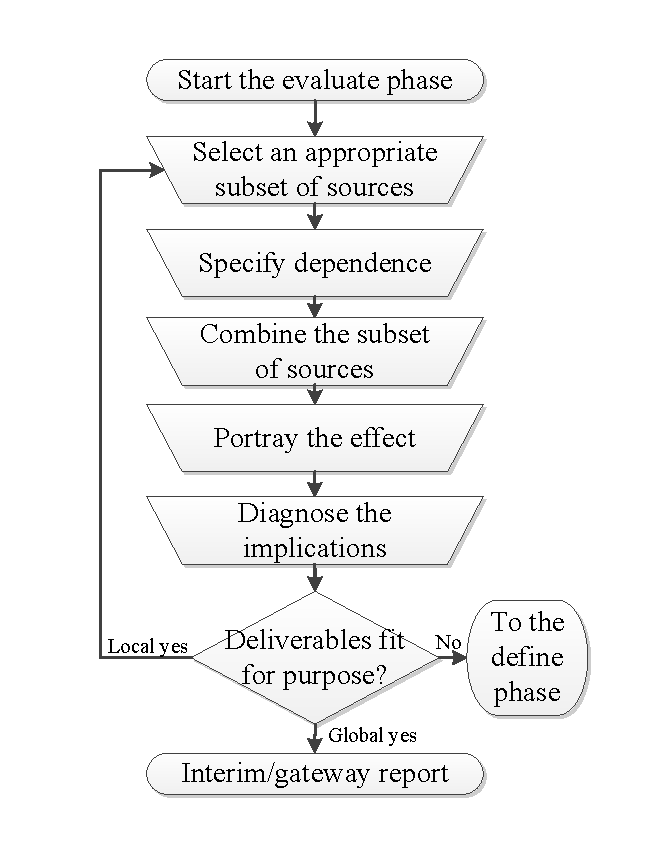
\includegraphics[width = 0.42\textwidth]{./Figures/Evaluate.pdf} 
\caption{Evaluate Phase Process - adapted from \cite{chapman}}
\label{Figure:Evaluate}
\end{figure}

Specifying dependence is an important mode of the phase.
To simplify the approach, many practioners following common practice may assume independence between sources.
This is an extremely dangerous assumption, and any formal analysis based on this on a non-evidential basis should be immediately discounted.
Falsely assuming independence paints an optimistic picture of the circumstances by ignoring the knock-on effects of underlying complexity.
This can be compounded by over-simplified computational tools that aim to make calculations easier, and by a managerial preference for limited variability. 
Positive dependence is a more reasonable assumption, making a more conservative, robust assessment of the impacts. 
In high-clarity contexts, complex statistical and causal dependencies may require more sophisticated modelling approaches to adequately understand the full implications.

The dangers of making false dependency assumptions is shown in the contrast between independent and positive correlation in figure \ref{Figure:ImpactsDependence}.
Two identical probability functions are combined by addition, showing the difference caused by dependence assumptions.
Any dependence relation between 0-100\% can be achieved by linear interpolation between the two curves.

\begin{figure}[!h]
  \centering
\subfigure[$C_{a}$ and $C_{b}$ probability density functions are identical]{
    \rule{7cm}{7cm} 
    %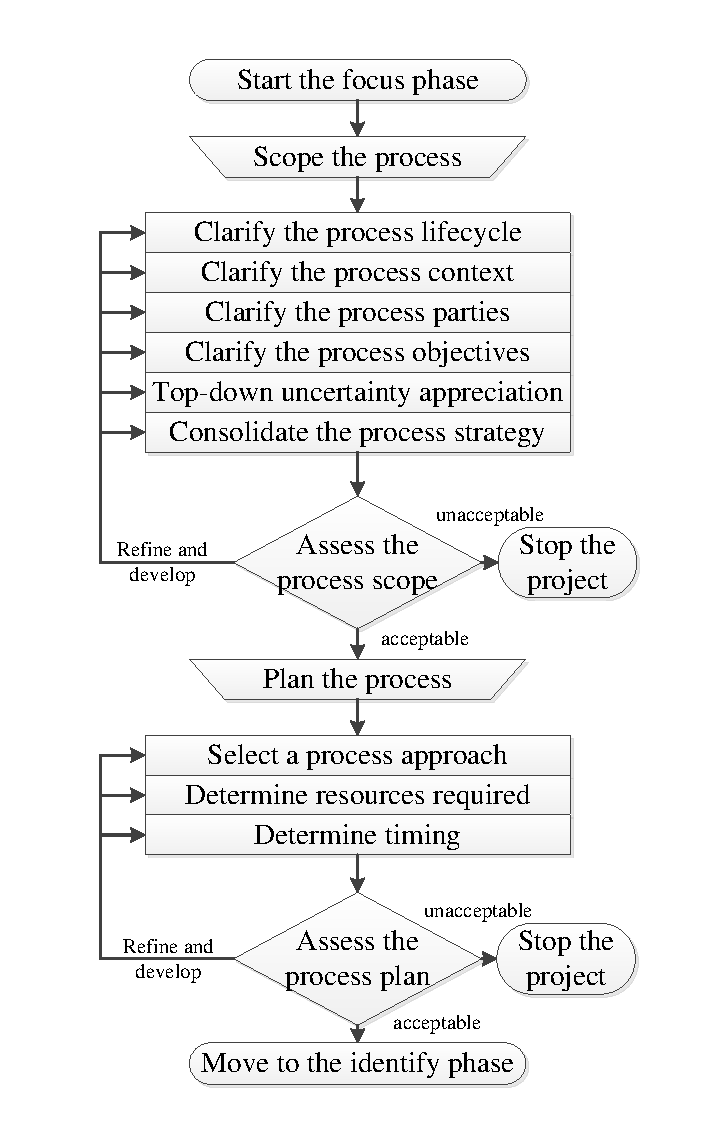
\includegraphics[height = 9.3cm]{./Figures/Focus.pdf}
	\label{Table:DepVals}
   } \quad
\subfigure[Combining $C_{a}$ and $C_{b}$ both independently $C_{i}$ and with positive dependence $C_{p}$]{
    \rule{7cm}{7cm}
    %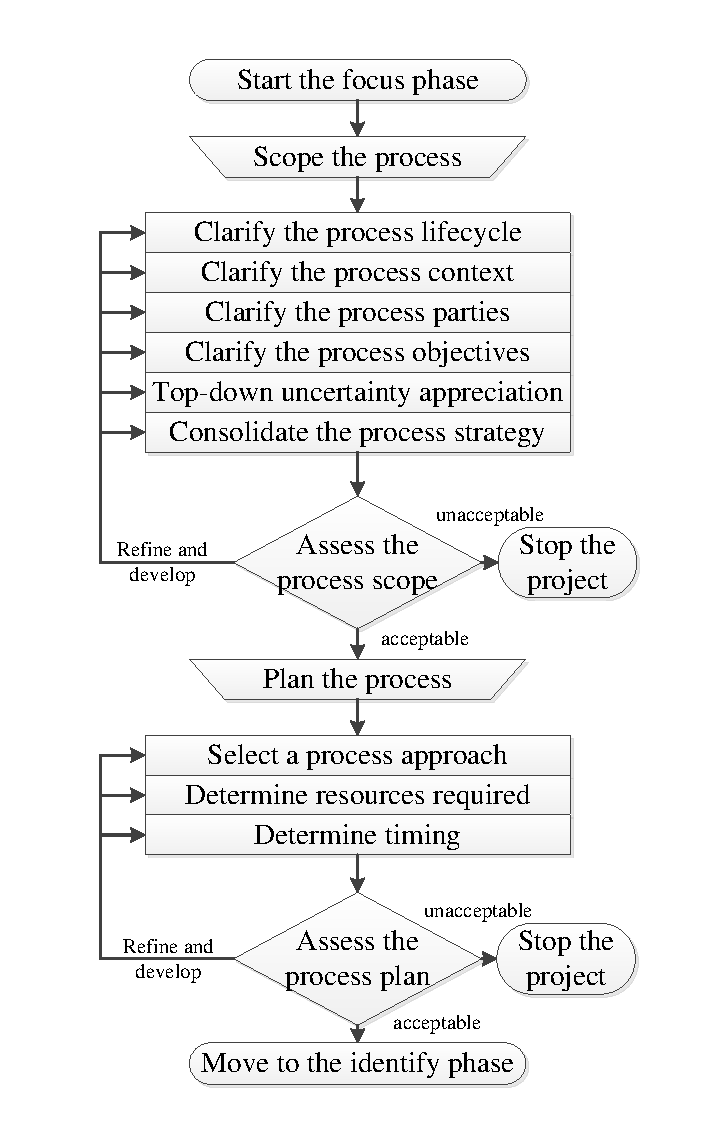
\includegraphics[height = 9.3cm]{./Figures/Focus.pdf} 
	\label{Figure:Dependency}
   }
\caption{The impacts of independent and positive dependence assumptions - adapted from \cite{chapman}}
\label{Figure:ImpactsDependence}
\end{figure}

Another key mode of the phase is to portray the effects. 
The story that has been developed throughout the analysis must be conveyed in the most clarity efficient manner to be of any practical value to the project organisation.
Sensitivity diagrams are an important tool for conveying and explaining uncertainty.
The common phrase ``a picture is worth a thousand words'' is relevant here.
A sensitivity diagram gives the audience the required information in a non-threatening easy-to-grasp format so that interpretation can take place and issues raised can be resolved.

The sensitivity diagram in figure \ref{Figure:SensDiag} shows the collation of five sources associated with the geotechnical investigations in preparation for the construction of a power station.
A diagram of this type may be required for each activity in a network.
The gap between each curve portrays the effect of the labelled source.
Four is clearly the most important source in this case. 
The ordering of the sources are important, so that causal and statistical dependence is portrayed by adjacency of sources.
A maximum of around six sources should be displayed on the diagram to ensure meaning remains clear.
Less important sources can be combined so that only the most relevant aspects of the story are shown.

\begin{figure}[!h]
  \centering
  \rule{5cm}{5cm}
    %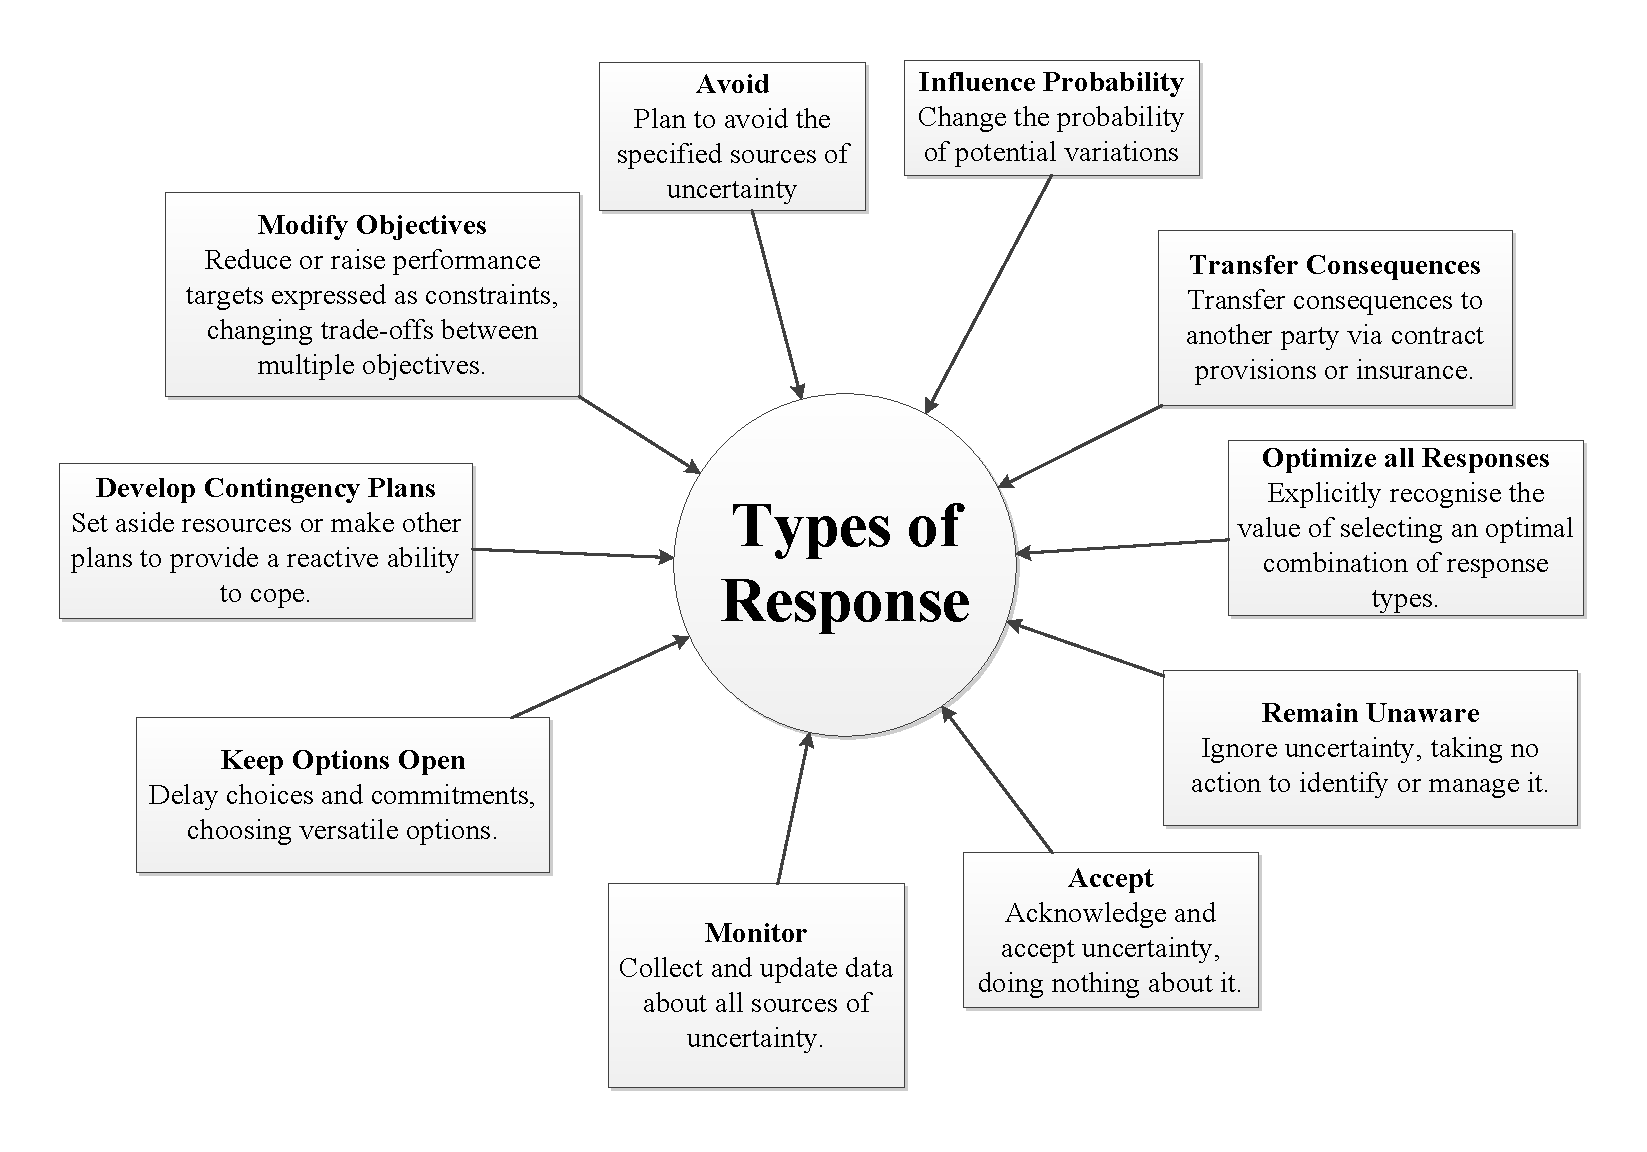
\includegraphics[width = \textwidth]{./Figures/ResponseTypes.pdf} 
\caption{Sensitivity diagram - adapted from \cite{chapman} \& \cite{hopkinson2008}}
\label{Figure:SensDiag}
\end{figure}

It may be useful to expand a sensitivity diagram where schedules are concerned. 
This can help develop a project strategy that includes realistic milestones and help identify contingency requirements \citep{hopkinson2008}.
Uncertainty can be decomposed through a number of project milestones and contracting activities.
This can be displayed alongside a Gantt chart to portray the schedule implications as in figure \ref{Figure:SensDiagGantt}.

\begin{figure}[!h]
  \centering
  \rule{5cm}{5cm}
    %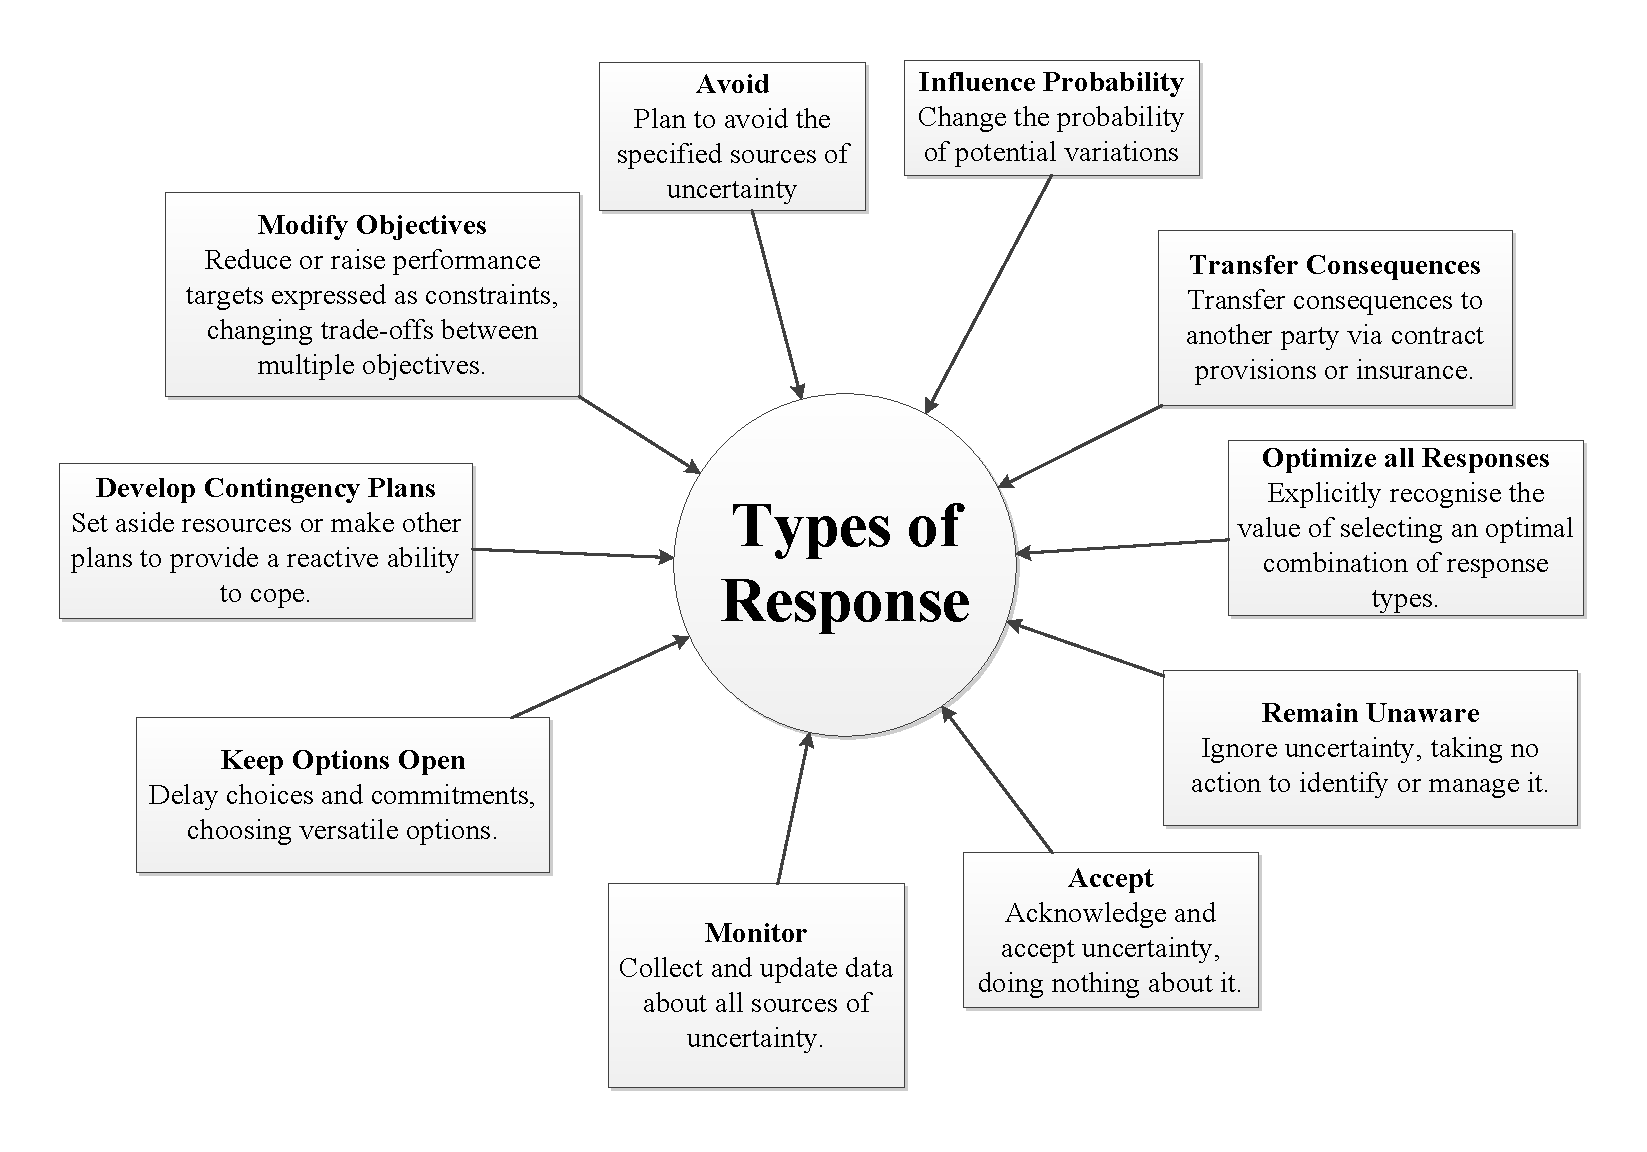
\includegraphics[width = \textwidth]{./Figures/ResponseTypes.pdf} 
\caption{Schedule sensitivity diagram - adapted from \cite{hopkinson2008} \& \cite{chapman} }
\label{Figure:SensDiagGantt}
\end{figure}

There are alternative forms of sensitivity diagram which may be useful for presenting uncertainty when there are several different parameters involved. 
One of these is the tornado diagram; a common output from Monte Carlo simulation programs.
Each parameter is varied in turn whilst the others are held at a constant expected value.
The sources are then portrayed in order of significance.

\begin{figure}[!h]
  \centering
  \rule{5cm}{5cm}
    %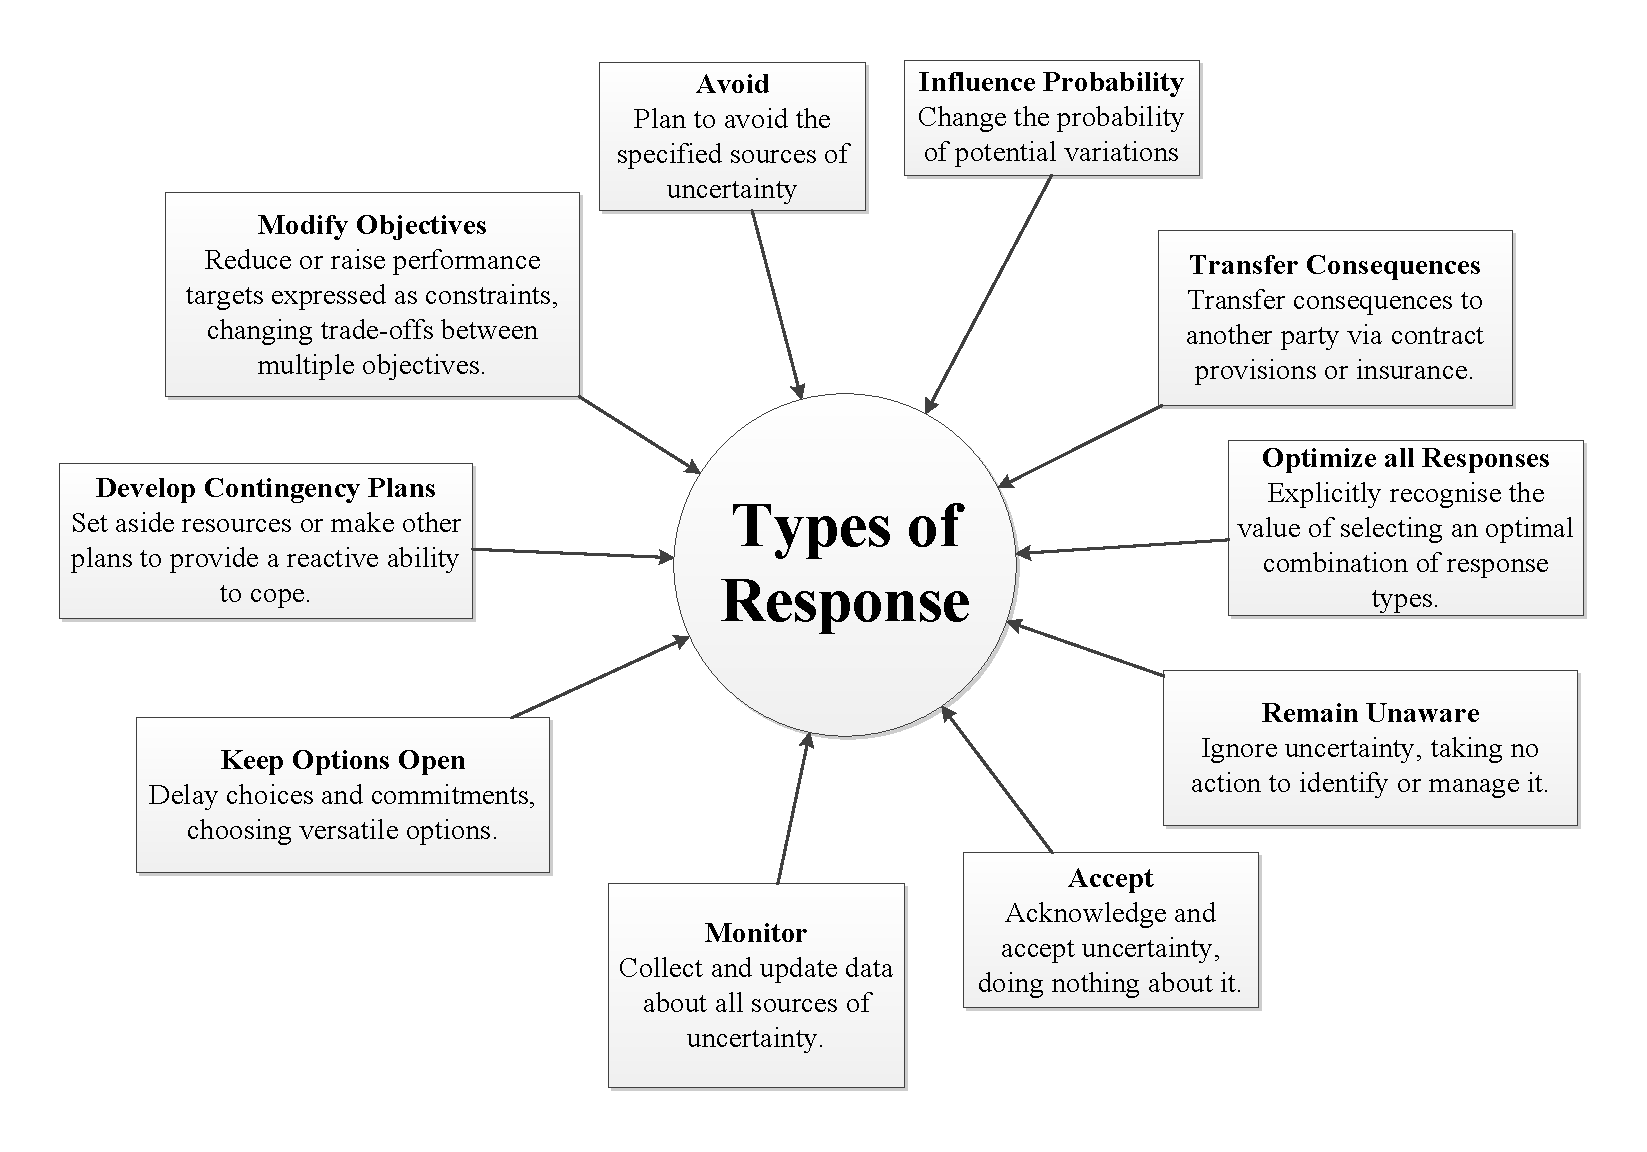
\includegraphics[width = \textwidth]{./Figures/ResponseTypes.pdf} 
\caption{Tornado diagram - adapted from \cite{hopkinson2008}}
\label{Figure:Tornado}
\end{figure}

The evaluate phase is key to the successful implementation of an iterative process.
Iteration is one of the key sources of clarity efficiency which is harnessed through the PUMP approach and the reason for special focus on the evaluate phase in this report.
It is essential that on the first pass of the PUMP that only a rough sizing of all relevant sources is undertaken.
The aim is not to achieve an accurate probability estimate for all sources; this is not clarity efficient and means time is not spent optimally.
The first pass should result in a simple order-of-magnitude picture of the importance of the sources so that successive iterations can refine the most important sources where useful.

Informed, effective and efficient decision taking is the key deliverable so that opportunity efficiency can be maximised.
The evaluate phase consolidates the outputs from the other phases for presentation and interpretation.
Attention must be paid to how dependency and assumptions are dealt with during this phase.
Any analysis that does not adequately consider these factors should be discounted.
The use of a nested structure of sensitivity diagrams together with decision diagrams \citep{chapman} highlights the trade-offs between sources.
This interpretation of the portrayed uncertainty culminates in the effective shaping of base plans and project strategy so that risk inefficiency is minimised while opportunity efficiency is maximised.




